
\documentclass{beamer}

\usepackage{color,soul}
\definecolor{lightblue}{rgb}{0.3,0.2,0.5}
%\setulcolor{lightblue}

\def\colorunderline#1#2#3{\color{#1}\underline{{\color{#2}#3}}\color{black}}

\usepackage{tikz}
\usepackage{setspace}

\usetikzlibrary{arrows}
\usetikzlibrary{decorations.markings}

% \usetikzlibrary{arrows.meta}

\usepackage{microtype}

\definecolor{lqboutercolor}{rgb}{.93,.91,.92}
\definecolor{lqbinnercolor}{rgb}{.98,.98,.98}

\definecolor{blGreen}{rgb}{.2,.7,.3}
\definecolor{darkRed}{rgb}{.2,.0,.1}

\definecolor{postLinkColor}{rgb}{.5,.5,.1}

\definecolor{fcBoxColor}{rgb}{.8,.6,.3}

\definecolor{BlueGreen}{rgb}{.1,.6,.4}

\newcommand{\colorbullet}[1]{{\color{#1}\ensuremath{\bullet}}}

\usepackage{setspace}
%\usetikzlibrary{arrows, positioning, shapes}
\usetikzlibrary{positioning, shapes}
%\usetikzlibrary{calc}

\newenvironment{tightcenter}{%
	\setlength\topsep{0pt}
	\setlength\parskip{0pt}
	\begin{center}
	}{%
\end{center}
}

\newcommand{\tightcenterline}[1]{\begin{tightcenter}#1\end{tightcenter}}

\tikzstyle{TextNode}=[shape=ellipse,double,draw=BlueGreen,fill=yellow!50,
text opacity=1,fill opacity=.6,text centered]

\tikzstyle{TextPolygonNode}=[shape=regular polygon,regular polygon sides=15,double,draw=BlueGreen,fill=yellow!50,
text opacity=1,fill opacity=.9,text centered,inner sep=0]

\tikzstyle{TextStarNode}=[shape=circle,double,draw=fcBoxColor,fill=black!20,
text opacity=1,fill opacity=.9,text centered,inner sep=2pt]

\usetikzlibrary{decorations.pathmorphing}

\tikzset{snake it/.style={decorate, decoration=snake}}

\tikzset{
	hv/.style={to path={-| (\tikztotarget)}},
	vh/.style={to path={|- (\tikztotarget)}},
}

%\tikzset{
%	strong arrow/.style={
%		decoration={markings,
%			%mark=at position 1 with {\arrow[scale=1,brown]{>}},
%			mark=at position 0.8 with {\arrow[>=stealth,scale=1.2,purple]{>};},
%			%mark=at position 1 with {\arrow[>=,scale=1.2,white]{>};} 
%			mark=at position 1 with {\arrow[>=stealth,scale=1.2,brown]{>};} 
%		},
%		postaction={decorate},
%		shorten >=1mm}}

%{-Triangle[angle=90:10pt,red,fill=blue]}

\begin{document}

\begin{frame}{\Huge{\textbf{Seamless Architecture}}}

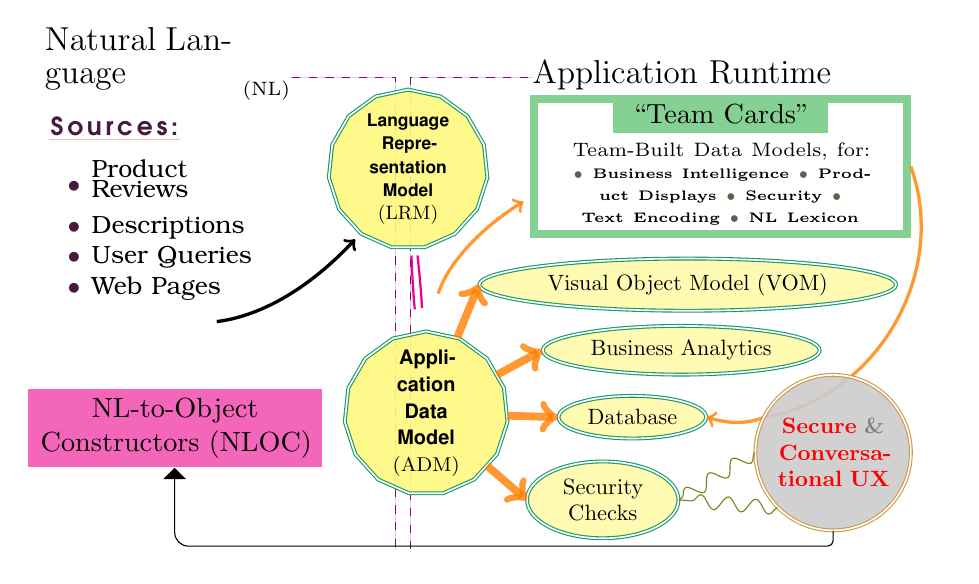
\begin{tikzpicture}%[node distance=1em]

%\node [rect={}{solid,draw=blue}{solid,draw=green,shorten >=\pgflinewidth}{solid,draw=orange,shorten <=-\pgflinewidth}] 
%(1) at (0,  0);

 
 %\node [rectangle={}{solid,draw=blue}{solid,draw=green}{solid,draw=orange}] (1) at (0,  0)  { $1$ };
 %\node [draw=red, draw opacity=0.5] (2) at (0.5,0)  { $2$ };



%  rect={}{solid,draw=blue}{solid,draw=green}{solid,draw=orange}
 \draw [purple,dashed] (0cm, -3cm) rectangle (2.9cm,3cm);
 \draw [purple,dashed] (3.1cm, -3cm) rectangle (6cm,3cm);

 \draw [blue,opacity=.2] (0cm, -3cm) rectangle (2.9cm,3cm);
 \draw [blue,opacity=.2] (3.1cm, -3cm) rectangle (6cm,3cm);

% \draw [blue,opacity=.2] (0cm, 3cm)--(2.9cm,3cm) ;
 \draw [white] (0cm, -3cm)--(0cm, 3cm) ;
 \draw [white] (0cm, -3cm)--(2.9cm, -3cm) ;

 \draw [white] (6cm, -3cm)--(6cm, 3cm) ;
 \draw [white] (6cm, -3cm)--(2.9cm, -3cm) ;

\path

node (LeftNode) (0cm, 0cm) {}
node (NaturalLanguageNode) at (0cm, 0cm) {}

node (CenterNode) at (current bounding box.center) {}

node (NaturalLanguageLabelNode) [above=27 mm of NaturalLanguageNode,
fill opacity=1,fill=white,text width=3.1cm, inner sep = 0] 
{\large{Natural Language}}


node (NaturalLanguageSourcesNode) [below=2 mm of NaturalLanguageLabelNode,
fill opacity=1,fill=white,text width=3cm] 
{\small{{\fontfamily{pag}\selectfont 
 \textls[150]{\textbf{\colorunderline{red!30}{black!80!blue!80!red!90}{Sources:}}} }
		{\fontfamily{pbk}\selectfont 
		\vspace{2mm} 
		\\ \hspace{1mm} \colorbullet{black!80!blue!80!red!90} \begin{minipage}{.8\textwidth}{\begin{spacing}{0.5}Product \\ Reviews\end{spacing}}\end{minipage} 
		\\ \hspace{1mm} \colorbullet{black!80!blue!80!red!90} Descriptions 
		\\ \hspace{1mm} \colorbullet{black!80!blue!80!red!90} User Queries 
		\\ \hspace{1mm} \colorbullet{black!80!blue!80!red!90} Web Pages
		
		}}}

node (NaturalLanguageLabelNodeNL) [right=-6 mm of NaturalLanguageLabelNode.east,
yshift = -4mm,
fill opacity=1,fill=white,inner sep = 0] 
{\scriptsize{(NL)}}


node (ConstructorsNode) [below=10 mm of NaturalLanguageSourcesNode,xshift=1mm,
fill opacity=1,fill=magenta!60,text width=35mm, text centered] 
{NL-to-Object Constructors (NLOC)}

node (TeamsNode) [right=4.1 cm of NaturalLanguageLabelNode,yshift = -7mm,
fill opacity=1,fill=blGreen!60,text width=25mm, text centered] 
{``Team Cards"}

node (TeamsNodeText) [below=0 mm of TeamsNode.north,
fill opacity=1,draw=blGreen!60, line width=1mm, text centered, minimum width=3cm, minimum height=1cm,
text width=4.5cm] 
{
 \vspace{4mm}
 \\
 \scriptsize{
 Team-Built Data Models, for: 
 \textbf{\tiny{\\
 \colorbullet{green!70!red!20!black!70} Business Intelligence  
 \colorbullet{green!70!red!20!black!70} Product Displays 
 \colorbullet{green!70!red!20!black!70} Security 
 \colorbullet{green!70!red!20!black!70} Text Encoding
 \colorbullet{green!70!red!20!black!70} NL Lexicon}}}
	
}


node (HiddenCenterNode) [right=1 mm of CenterNode] {}

node (HiddenLeftNode) [right=30 mm of HiddenCenterNode] {}

node (ApplicationDataNode) [above=27 mm of HiddenLeftNode,fill opacity=1,fill=white, inner sep = 0] 
{\large{Application Runtime}}

node (ApplicationDataModelNode) [TextPolygonNode,minimum height=2cm,minimum width=1cm,
 below=1 mm of HiddenCenterNode,
 text width=12mm,inner sep=-1mm,scale=.8] 
{\textbf{\small{{\fontfamily{phv}\fontseries{b}\selectfont Appli\-cation Data Model}}} \small{(ADM)}}

node (LanguageRepresentationNode) [TextPolygonNode,
 above left = 10 mm and -6 mm of HiddenCenterNode,
text width=17mm,scale=.7,inner sep=0mm] %,minimum height=1cm,inner sep=-1mm,scale=.8] 
{\textbf{\small{{\fontfamily{phv}\fontseries{b}\selectfont Language Representation Model}}} (LRM)}

node (HiddenDataComponentsNode) [right=1 mm of ApplicationDataModelNode] {}

node (DatabaseNode) [TextNode,right=3 mm of HiddenDataComponentsNode,
 yshift = -0.5mm,
 scale=.8] %,minimum height=1cm,inner sep=-1mm,scale=.8] 
{Database}

node (SecurityNode) [TextNode,right=-1 mm of HiddenDataComponentsNode,
yshift = -11mm, text width = 1.5cm, inner sep=1mm,
scale=.8] %,minimum height=1cm,inner sep=-1mm,scale=.8] 
{Security Checks}

node (DatabaseNodeOrient) [right=5 mm of DatabaseNode] {}
node (DatabaseNodeOrientE) [right=6 mm of DatabaseNode,yshift=0.5mm] {}

;

\draw [ -, very thick, draw=orange, opacity=.8, bend left=50,looseness=1,
shorten >= 0mm, shorten <= 0mm ] 
(TeamsNodeText.east) to (DatabaseNodeOrient.east); 

\draw [ % strong 
 ->, very thick, draw=orange, opacity=.8, bend left=20,looseness=1,
shorten >= 0mm, shorten <= 1mm ] 
(DatabaseNodeOrientE.east) to (DatabaseNode.east); 

\path


node (ConversationalUXNode) [TextStarNode,right=28 mm of HiddenDataComponentsNode,
yshift = -5mm, scale=.8, text width=2cm] %,minimum height=1cm,inner sep=-1mm,scale=.8] 
{\color{red}{\textbf{Secure \color{gray}{\&} \color{red}{Conversational UX}}}}

node (BusinessAnalyticsNode) [TextNode,right=1 mm of HiddenDataComponentsNode,yshift = 8mm,scale=.8] %,minimum height=1cm,inner sep=-1mm,scale=.8] 
{Business Analytics}

node (VisualObjectModelNode) [TextNode,above right=1mm of HiddenDataComponentsNode,yshift = 12mm, scale=.8] %,minimum height=1cm,inner sep=-1mm,scale=.8] 
{Visual Object Model (VOM)}

%{\begin{spacing}{1.0}\tightcenterline{Application Data Model (ADM)}\end{spacing}}}
;

%\draw [ strong arrow, very thick, opacity=.8, line width=1mm 
 %bend right=30,looseness=1 
% ] (ApplicationDataModelNode) edge (DatabaseNode.south); 


%\draw [ strong arrow, very thick, draw=orange, opacity=.8, line width=1mm, 
%bend right=30, looseness=1 
% ] (ApplicationDataModelNode) to (DatabaseNode.south); 

\draw [ % strong arrow,
  ->, very thick, draw=orange, opacity=.8, line width=1mm] 
(ApplicationDataModelNode) to (DatabaseNode.west); 

\draw [ % strong arrow, 
  ->, very thick, draw=orange, opacity=.8, line width=1mm] 
(ApplicationDataModelNode) to (SecurityNode.west); 



\draw [ % strong arrow, 
 ->, very thick, draw=orange, opacity=.8, line width=1mm,
%bend right=2,looseness=4,shorten >= 2mm 
] (ApplicationDataModelNode) to (BusinessAnalyticsNode.west);

\draw [ % strong arrow, 
 ->, very thick, draw=orange, opacity=.8, line width=1mm] (ApplicationDataModelNode) to (VisualObjectModelNode.west); 


\draw [ ->, very thick, bend right=20,looseness=1,shorten >= 1mm, shorten <= 5mm ] node [below=1mm of 
NaturalLanguageSourcesNode.south] {} edge (LanguageRepresentationNode); 


\draw [ % strong arrow, 
  ->, very thick, draw=orange, opacity=.8, bend left=20,looseness=1,shorten >= 1mm, shorten <= 5mm ] (ApplicationDataModelNode.north) 
 to (TeamsNodeText); 

%\draw [ strong arrow, very thick, draw=orange, opacity=.8, bend left=100,looseness=1,shorten >= 1mm, shorten <= 5mm ] 
%(TeamsNode.east) to (DatabaseNode.east); 


%\draw [ -> , draw=orange, shorten <= 3mm , thick, scale=4] (LanguageRepresentationNode) edge (ApplicationDataModelNode); 
%\draw [orange, strong arrow ] (LanguageRepresentationNode) to (ApplicationDataModelNode); 


 %? \draw [orange, line width=2mm,arrows={-Triangle[angle=90:10pt,black!80,fill=orange]}] (LanguageRepresentationNode) to (ApplicationDataModelNode); 

\path
node (ArrowTop) [above = 3mm of LanguageRepresentationNode.south] {} 
node (ArrowBottom) [left = 2mm of ConstructorsNode.north east] {} ;

%? \draw [orange, opacity=.4, line width=2mm, shorten <= 5mm, shorten >= .5mm, arrows={-Triangle[angle=90:10pt,black!80,fill=orange]}] 
%?  (ArrowTop) to (ArrowBottom); 

%\draw [ - ,bend left=2,looseness=1, draw=magenta, thick,
%shorten <= 5mm, shorten >= 3mm ] (ArrowTop) edge (ArrowBottom); 
%\draw [ - ,bend right=2,looseness=1, draw=magenta, thick,
%shorten <= 5mm, shorten >= 3mm ] (ArrowTop) edge (ArrowBottom); 
%\draw [ - %,bend left=5,looseness=1, 
%, line width=14mm,
%draw=white, opacity = .3, thick,
%shorten <= 2mm, shorten >= 3mm ] (ArrowTop) edge (ArrowBottom); 

%? \draw [orange, opacity=.4, line width=2mm, shorten <= .3mm, shorten >= 8mm, %? arrows={-Triangle[angle=90:10pt,black!80,fill=orange]}] 
%? (ConstructorsNode.north east) to (ApplicationDataModelNode.center); 

%\draw [ - ,bend left=2,looseness=1, draw=magenta, thick,
%shorten <= 5mm, shorten >= 3mm ] (ConstructorsNode.north east) edge (ApplicationDataModelNode.center); 
%\draw [ - ,bend right=2,looseness=1, draw=magenta, thick,
%shorten <= 5mm, shorten >= 3mm ] (ConstructorsNode.north east) edge (ApplicationDataModelNode.center); 
%\draw [ - %,bend left=5,looseness=1, 
%, line width=14mm,
%draw=white, opacity = .3, thick,
%shorten <= 2mm, shorten >= 3mm ] (ArrowTop) edge (ArrowBottom); 



\draw [ - %,bend left=5,looseness=1, 
 , line width=14mm,
 draw=white, opacity = .3, thick,
shorten <= 2mm, shorten >= 3mm ] (LanguageRepresentationNode) edge (ApplicationDataModelNode); 

%\draw [ - ,bend right=5,looseness=1, draw=cyan!40, thick,
%shorten <= 2mm, shorten >= 3mm  ] (LanguageRepresentationNode) edge (ApplicationDataModelNode); 

\draw [ - ,bend left=2,looseness=1, draw=magenta, thick,
 shorten <= 1mm, shorten >= 3mm ] (LanguageRepresentationNode) edge (ApplicationDataModelNode); 

\draw [ - ,bend right=2,looseness=1, draw=magenta, thick,
 shorten <= 1mm, shorten >= 3mm ] (LanguageRepresentationNode) edge (ApplicationDataModelNode); 

\draw [hv, ->, >=triangle 90, rounded corners=5pt] 
 node (temp) [below left = 1mm of ConversationalUXNode.south] {} edge (ConstructorsNode.south);

\draw [hv,rounded corners=2pt] 
 (temp.west) edge (ConversationalUXNode.south);
 
\path [draw=postLinkColor,snake it]
(ConversationalUXNode.south west) -- (SecurityNode.east);

\path [draw=postLinkColor,snake it]
(ConversationalUXNode.west) -- (SecurityNode.east);

%\draw[draw=blue, snake it] (2,0) arc (0:180:2cm);
 
%\draw [-, snake it ] (ConversationalUXNode.west) edge (SecurityNode);

%\node [rectangle={}{draw=red}{draw=red}{}] at (0cm, 0cm) {NN};

%\node [rect={solid,draw=blue}{}{solid,draw=green}{solid,draw=orange}] at (0cm, 0cm) {NN};


\end{tikzpicture}

\end{frame}

\end{document}
